% Publication-only edition. RD1 at 050e4f4 and every prior file are unchanged.
\documentclass[10pt]{article}
\usepackage[margin=0.85in]{geometry}
\usepackage{amsmath,amssymb,booktabs,array,longtable,graphicx,hyperref,microtype}
\hypersetup{hidelinks,pdftitle={History dependence without qualified common support},pdfauthor={networkRLCD project}}
\setlength{\emergencystretch}{2em}
\graphicspath{{../../reports/figures/}}
% Rounded existing report values only. No reanalysis or model search.
\newcommand{\NVNinePSNR}{0.508}
\newcommand{\NVNinePSNRLow}{0.077}
\newcommand{\NVNinePSNRHigh}{0.938}
\newcommand{\NVTenDelta}{-14.1}
\newcommand{\NVTenLow}{-22.6}
\newcommand{\NVTenHigh}{-5.5}
\newcommand{\MFiveKampar}{0.20746}
\newcommand{\MFiveKamparLow}{0.09910}
\newcommand{\MFiveKamparHigh}{0.31413}
\newcommand{\MFiveVolga}{0.14750}
\newcommand{\MFiveVolgaLow}{0.09807}
\newcommand{\MFiveVolgaHigh}{0.19353}
\newcommand{\POOneTable}{%
\begin{table}[ht]
\centering\small
\begin{tabular}{lrrrrrr}\toprule
&\multicolumn{3}{c}{Factual BWE MAE (octaves)}&\multicolumn{3}{c}{Synthetic advantage MAE}\\
Family&Persistence&S1&H1&Constant&S1&H1\\\midrule
sawtooth & 0.740 & 0.457 & 0.469 & 0.256 & 0.204 & 0.203\\
square\_wave & 0.684 & 0.413 & 0.421 & 0.251 & 0.200 & 0.199\\
slow\_fade & 0.587 & 0.447 & 0.469 & 0.183 & 0.152 & 0.154\\
feedback\_flap & 0.407 & 0.716 & 0.724 & 0.080 & 0.221 & 0.225\\
\bottomrule\end{tabular}
\caption{PO1 frozen validation values: 72 episodes/family across three fixed fits, six nested decisions/episode. S1 is the fixed-history summary baseline; H1 adds ordered lags. Lower is better. These are simulator results, not native effects.}\label{tab:po1}
\end{table}}

\title{History dependence without qualified common support:\\
Limits of learned native bitrate control}
\author{networkRLCD project\\Retrospective research-decision synthesis}
\date{15 October 2026 --- publication edition; scientific decision fixed at RD1}
\begin{document}
\maketitle

\begin{abstract}
% claim: abstract
Fine-grained learned bitrate control requires a defensible connection between
sender information, randomized action effects and future delivery risk. We
synthesize frozen native Chromium and simulator studies that did not establish
that connection robustly. Two bounded native causal findings anchor the result:
randomized early service history changed later bandwidth estimates (BWE), and
a fixed BWE-threshold policy reduced timely delivery by 14.1 percentage points
(unadjusted 95\% interval $[-22.6,-5.5]$) relative to fixed 0.65. A positive
secondary quality interaction in a local action study did not receive an
adequately covered independent replication. Subsequent support studies did not
establish reproducible conditional native state. History effects varied with
content and time; no registered sustained convergence was found by 36 s.
Available mechanism channels failed their discrimination criteria. Internal
transport events existed, but their online freshness and identity did not
jointly qualify; a proposed instrumented fixture was never built because
resource admission failed. Separately, an 816-episode simulator screen failed
robust out-of-family prediction and action discrimination. Interval coverage
met its registered minimum, but excessive width and failed probability
calibration prevented useful supported uncertainty. Its native factual panel
remains unopened. These findings support RD1's stopping decision under the
available fixture/data assumptions. They do not establish universal control
impossibility, permanent history memory, or the irrelevance of observable
history. No successor, additional model or controller is introduced.
\end{abstract}

\section{Research question and contribution}
% claim: motivation
Interactive media must balance source quality, timely delivery and network cost;
these goals are not interchangeable~\cite{rfc8836}. A native sender's reported
bandwidth estimate (BWE) is an output of a transport/encoder feedback system,
not an exogenous measurement of usable capacity. A controller could exploit
observable history only if its action-value and risk claims are identifiable
for the relevant population and survive validation. Good mean prediction in one
regime is insufficient; useful uncertainty must also transport~\cite{ovadia}.

% claim: contribution
The original networkRLCD program investigated calibrated learned adaptation in
simulation, then native action effects and causal support. Its evidence anchor
is commit \texttt{f109ab2}, the completed PO1 result. Its scientific stopping
decision is RD1 at \texttt{050e4f4}~\cite{rd1}; this publication pass changes
neither evidence nor decision. All prior artifacts, including the earlier
controller-centric manuscript and the RD1 edition, are preserved.

The central contribution is an empirically delimited failure to connect local
causal effects to reproducible conditional control value. Bounded causal history
effects and local policy harm were observed. Reproducible conditional native
state, internal causal observability, robust synthetic action discrimination and
useful calibrated uncertainty were not established. Each failed link has its own
experimental unit, gate and scope. This separation preserves what was learned
without treating a support failure as an action outcome or inaccessible state
as an irrelevant mechanism. The result is a stopping decision under explicit
assumptions, not a controller or safety certificate.

% claim: earlier_simulation
Earlier simulator studies retain their reported local successes and failures
in the frozen prior edition~\cite{earlier}. They used different representations,
policies and targets; PO1 does not erase those results or supply their native
validation. Passing some synthetic population-panel criteria did not establish
uniform within-family calibration or native control value.

\section{Estimands and what failure means}
\label{sec:estimands}
% claim: estimands
Let $\mathcal I_t$ contain sender observations, past commands and records
\emph{actually received} by decision time $t$. Let $U_t$ denote unobserved
transport state, $A_t$ a bitrate action and $Y$ a specified future endpoint.
Three questions must remain separate:
\begin{align}
\tau_H(t;S)&=\mathbb E[X_t(H_d,S)-X_t(H_a,S)],\\
\tau_A(s;\mu)&=\mathbb E_{\mu}[Y(a_1)-Y(a_0)\mid g(\mathcal I_t)=s],\\
V_{\mu}(\pi)-V_{\mu}(\pi_0)&=\mathbb E_{\mu}[Y(\pi)-Y(\pi_0)].
\end{align}
The first is a total effect of randomized early service order $H$ followed by
common input service $S$. For M5, $X_t$ is the mean log2-BWE response over the
registered eleven observations, with the fixed normalization specified below.
The second is a conditional action effect under a
specified history/episode distribution $\mu$. The third is a complete policy
or sequence contrast. A factual predictor
$\mathbb E[B_{t+1:t+h}\mid\mathcal I_t,\text{logging regime}]$ is a fourth,
predictive target; it is not a native counterfactual action value.

% claim: identification
Randomized actions can identify local or marginal effects despite hidden
$U_t$, subject to consistency, actual randomization/positivity and the stated
population. Observing every GCC mechanism or finding a stationary Markov state
is not a universal prerequisite for randomized policy inference. Native V9 and
V10 demonstrate that bounded causal contrasts can be estimated in this fixture.
The project's intended \emph{transferable fine-grained conditional value},
however, additionally needs support and a defensible relationship between
the selected observable context and its future response across histories and
sources. That relationship has not qualified. Changing $\mu$ can change the
latent-history mixture even when instantaneous BWE is the same~\cite{rd1}.

% claim: classifications
We distinguish a supported bounded causal effect, a contradicted specific
superiority claim, an unsuccessful registered recipe, an unestimable comparison
after a gate failure, a fixture/practical limit, and an unresolved mechanism.
None alone is a theorem that all learned native control is impossible. Failed
support sessions are not treatment outcomes; zero emitted predictions have
unestimable precision. Receiver outcomes left unopened in support studies are
not assigned zero effects.

\section{Evidence handling, sources and technical controls}
\label{sec:evidence}
% claim: evidence_handling
This is a synthesis of committed result reports and their pinned provenance,
not a meta-analysis or raw-data reanalysis. No captures are restored, no closed
validation representation is searched, no receiver outcome is opened and no
new model is fitted. RD1's evidence ledger binds cited reports, protocols and
selected storage receipts to SHA-256. The publication claim map adds exact
source locators, classifications and independence units. A preservation audit
checks every file tracked at the publication baseline, including RD1. This
edition is separate so that old scientific freezes remain valid.

% claim: source_scope
Native Chromium outcomes, native responses to controlled synthetic service,
measured-rate replay and simulated outcomes are distinct. Native V9/V10 used
generated content and a controlled schedule; their native telemetry is not a
fluid simulation. V11D crossed licensed source content with four strata nested
in two measured campaigns. V12 used three campaigns. V13's LTE/EVDO bundles
come from one measurement program. M5 onward reuse licensed content and
measured-source apparatus; many later common-service plateaus are controlled
inputs. A fresh browser process is a fresh run, not a new independent content
production or network campaign. Measured application-throughput replay is not
a live Internet trial or an observation of every end-to-end queue~\cite{v9,v10,v11d,v12,v13,m5,m8,m9r}.

% claim: technical_controls
The managed browser policy prohibits nonproxied UDP. Qualified native acquisition
used TURN/TCP without changing that policy. Sender/relay clock markers,
actual-run held-out clock coverage, native initialization, cap/jitter readback,
replay fidelity and cleanup were enforced before admitted analyses. Later
receipt-based features could not use future clock anchors or backdated event
timestamps. Technical qualification is necessary for attribution, but is not
scientific common support. Original failures and prospective repairs remain
separate studies~\cite{v9,v10,m5,m6r,m11r}.

\section{Native action evidence did not establish transferable value}
\subsection{A local secondary signal and a harmful policy}
% claim: native_v9
Ratios 0.65 and 1.05 denote multiples of pre-action sender BWE.
Native V9 randomized these BWE-relative caps at six 3 s boundaries in 48
sessions, nested in 12 generated-scene seed clusters. Its high/low BWE split
was prospectively fixed at 500 kbps. Eleven clusters met the
registered state/action counts; one remained in the evidence but outside the
complete-cell analysis. The primary high-minus-low BWE interaction in the 150 ms
on-time fraction was $-1.8$ percentage points, with an unadjusted 95\% $t$ interval
$[-29.4,25.8]$. The secondary PSNR interaction was
$\NVNinePSNR{}$ dB $[\NVNinePSNRLow{},\NVNinePSNRHigh{}]$~\cite{v9}.
Both intervals use 11 seed-cluster contrasts (10 degrees of freedom); holds
and frames are not independent replicates. PSNR is sampled among on-time frames,
not common-frame quality under all actions or human QoE. This supports a local
secondary signal under that logging regime, not a stable state value or policy
benefit. The primary delivery interaction remains unresolved.

% claim: native_v10
Native V10 tested the direct whole-session policy implication: use 1.05 at or
above the frozen 500 kbps BWE boundary and 0.65 below, versus fixed 0.65.
All 48 sessions qualified; two repeats/policy were averaged within each of
12 scene seeds. The threshold policy's on-time contrast was $\NVTenDelta{}$
percentage points $[\NVTenLow{},\NVTenHigh{}]$. PSNR was $+0.257$ dB
$[-0.132,0.646]$. Policy assignment was for a whole session; the delivery
endpoint was the 150 ms on-time frame fraction over six registered 800 ms
post-acknowledgment windows. Both intervals are unadjusted 95\% paired $t$
intervals over 12 scene-seed contrasts (11 degrees of freedom), not 48 independent
source units~\cite{v10}. The specific threshold policy's local superiority claim
is contradicted. This policy is closed and is not retuned. A positive local
quality interaction did not translate into whole-session policy benefit.

\subsection{Under-covered replication and action stages that never opened}
% claim: v11d
V11D completed 64 qualified native captures from four content groups, four
network-family strata and two measured campaigns. Only 9/16 crossed cells had
at least two holds in every state/action bucket; at least 13 were required.
Only seven cells had PSNR in every bucket, also below the required 13
primary-estimable cells. Their descriptive PSNR interaction was $-0.609$ dB,
with campaign means $-0.419$ dB (NordicDat) and $-0.862$ dB (Rome), from four
and three primary-estimable cells respectively~\cite{v11d}. Both directions
oppose V9, but the coverage gate failed. This is a negative, under-covered
replication, not a population reversal estimate. No missing bucket is imputed;
16 crossed cells and four nested families are not independent campaigns.

% claim: v12
V12 attempted all 24 support originals before randomizing any action.
Twenty-three ordinary captures sealed and one preserved capture failed native
media statistics. Ten passed all gates; none of six cells had complete frozen
low/high-BWE support. The 23 ordinary captures passed clocks, transport, replay
and cleanup. All 48 planned action sessions stayed unrun~\cite{v12}.
The six cells are two content groups $\times$ three campaigns, with two support
checks per state per cell. Capacity-based source hints did not guarantee native
estimator occupancy. The failed original is not counted as technically qualified.

% claim: v13
V13 replaced the binary split with a preregistered continuous BWE interaction,
but still required support before actions. All 32 originals individually
qualified. Six of 16 content/profile contexts exceeded the 0.25-octave fresh-repeat
limit; only one of four cells passed completely. All cells passed profile range
and SD, yet the cross-cell support intersection was empty. The 16 contexts are
two contents $\times$ eight profiles, with two repeats each; the four cells are
content $\times$ replay family. Its 64 randomized action sessions remain
unrun~\cite{v13}. V12/V13 supply no action-effect or QoE result. Individual
technical qualification cannot substitute for panel support.

\section{History is causal; usable common state did not qualify}
\subsection{M5's supported finite-history effect}
% claim: m5_design
M5 qualified 84 original sessions and 42 randomized prefix pairs before its causal
comparison. Within each of two reused contents, 21 adjacent pairs received
ascending/descending permutations of the same early service multiset and then
the same measured-source suffix. Actual-run clocks and suffix-exposure checks
passed~\cite{m5}.

% claim: m5_effect
At 18 s, descending-minus-ascending mean log2-BWE differences were
$\MFiveKampar{}$ octave $[\MFiveKamparLow{},\MFiveKamparHigh{}]$ for Kampar and
$\MFiveVolga{}$ $[\MFiveVolgaLow{},\MFiveVolgaHigh{}]$ for Volga.
Both registered distribution tests reject at local $\alpha=0.025$. The endpoint
is an eleven-sample mean of $\log_2(\mathrm{BWE}/500000)$; normalization is not a
binary threshold. Brackets are 95\% paired-bootstrap intervals from the frozen
10,000-draw procedure, using 21 randomized pairs per content. The exact paired
distribution tests and mean intervals answer different questions. Contents and
studies are not pooled; intervals describe repeated fixed-recipe capture
uncertainty, not a new-source population~\cite{m5}.

% claim: m5_scope
Later signed effects changed direction and neither content satisfied sustained
convergence through 36 s. Thus early service history causally changes later native
BWE in this fixed recipe. This does not establish permanent memory, behavior
beyond the horizon, independent network replication, or a unique mediator.
Holding later service input common does not force identical internal queue,
encoder or estimator trajectories. These are two reused contents and one reused
LTE measurement source~\cite{m5}.

\subsection{Matching, conditioning and dynamic-state failures}
% claim: m6r
M6R qualified 32 originals but only four of six frozen content/landmark strata
met membership coverage. Adding recent encode-time history excluded zero
BWE-only matches; the selected state had exactly the baseline membership.
Conditional future comparisons were therefore not run~\cite{m6r}. The six strata
are two contents $\times$ three landmarks; eight originals/history/content
share those landmarks. This is sparse overlap and absent matching discrimination
at the frozen calipers, not a null causal history effect. Conditioning on
post-prefix BWE/history cannot by itself identify a direct prefix effect or
causal mediation.

% claim: m7ra
M7RA's four feasibility originals passed technical gates, but only two reached
the instantaneous target and one met sustained-history membership. Neither
region qualified across histories. Its 128-session validation remains
untouched~\cite{m7ra}. The four contexts use one reused content, two targets and
two histories, with one original per context. These are deterministic gate checks,
not population rates; the larger validation requirements were never assessed.
A fixed conditioning recipe did not create common state.

% claim: m8_dynamics
M8's 16 characterization originals under repeated 24 s controlled-service plateaus
showed strongly asymmetric native dynamics: rise t50 about 7.4--10.2 s and t90
13.3--15.9 s, versus fall t50 about 0.39--0.79 s. These are envelopes of
input-normalized onset intervals across observed contexts, including sampling
and input-clock uncertainty, not population confidence intervals or time to an
assumed equilibrium. The 16 runs cross two reused contents, two prefixes, two
initial orders and two repeats; two earlier instrumentation originals qualified
separately~\cite{m8}. These are native content/encoder/transport responses to
controlled service, not simulated BWE or isolated GCC parameters.

% claim: m8_settling
At each frozen candidate age (6, 9, 12 and 15 s), none of 64 plateau occurrences
was future-verified under the D1 local-settling rule. The occurrences are four
plateaus nested in each of 16 native runs. D1 emitted some tags, but none verified;
no conditioning age was selected~\cite{m8}. The onset search is censored and
cannot prove permanent nonsettling.

% claim: m9r
M9R prospectively extended observation to a 64 s common plateau; all eight
instrumentation and 64 validation originals qualified. Instantaneous BWE (B0)
tagged 64 originals and D1 tagged 55, with no future-verified first predictions.
The phase-aware P2 rule emitted no tag, making its positive precision
unestimable. Full four-pair matching coverage fell from 42/64 strata for
BWE-only to 13/64 for the compact history vector. Residual future divergence
remained in some matched contexts~\cite{m9r}. Validation crosses two reused
contents, four service inputs, two histories and four repeats/history.
The 64 matching strata cross two contents, four inputs and eight landmarks;
landmarks share runs. There were zero future-stability labels in 3,200 nested
run/grid queries, not 3,200 independent experiments. Longer observation did not
establish prospectively useful state; it does not license another wait or
classifier on these closed captures.

\section{Mechanism observability and build practicality}
\subsection{M10R: available counters did not resolve residual divergence}
% claim: m10r
M10R qualified four instrumentation and eight fresh development originals at
1.414 Mbps common input. It observed acknowledged owned-relay queue/service
counters, native RTCP RTT, RTT-counter detection age, send/cap history and
encoder behavior. No channel met the frozen repeated same-direction contrast
with controls in both contents. Of 96 nested pair/landmark contrasts, 49
compact-matched; 23 of those 49 exceeded the 0.25-octave future-distance bound.
The eight development runs are two reused contents $\times$ two histories
$\times$ two repeats. Repeated landmarks and prepaired/crossed/within-history
contrasts share those runs. There were 0/400 positive future-stationary labels,
nested in eight originals; no stability classifier was fitted~\cite{m10r}.

% claim: m10r_scope
RTT-counter detection age is not transport-CC generation/arrival age; the owned
relay is one queue, not every queue in the TURN/TCP path. Available contrasts
may be consequences of BWE or shared causes. Seven of 14 compact-matched
within-history comparisons also diverged, so residual variability is not all
an isolated prefix effect. The assay established neither causal mediation nor
a stationary or prospectively reproducible trajectory state. Some repeatable
moving marginal distributions are insufficient~\cite{m10r}.

\subsection{M11R: real events lacked jointly useful freshness and identity}
% claim: m11r_channels
Both M11R native capability originals qualified ordinary acquisition. Identified
RTC logs contained actual TCC, delay/loss estimator-update and probe events.
The gate required at least 90\% of each event family sender-available within
250 ms in each original, clock uncertainty at most 50 ms, no continuous-feedback
delivery gap above 1,000 ms and stable PC/SSRC/controller attribution. Fresh TCC
counts were 31/1,739 (1.78\%) and 33/1,747 (1.89\%); fresh BWE-update counts
30/2,110 (1.42\%) and 37/2,090 (1.77\%); fresh probe counts 0/16 and 0/31.
Events are nested in two capability originals, not independent trials.
First identified export was about 59 s after measurement start, followed by
roughly 5 s batches~\cite{m11r}.

% claim: m11r_limit
Verbose target-update lines were fresh but lacked controller identity; a target
emission is not every estimator update. Trace exports supplied no online sender
receipt. No relay/socket/RTT/RTP-burst equivalent proxy qualified. All required
channels qualified in 0/2 originals. A record becomes causally usable at its
receipt, not its earlier producer timestamp. Full internal pacer queue/credit/cwnd
and probe-active state were not obtained. Transport-timing explanations of
residual divergence remain untested in this fixture, not disproved~\cite{m11r}.

\subsection{IF1: the instrumented alternative was not built}
% claim: if1
IF1 specified pinned Chromium/WebRTC hooks, stable identity, nonblocking event
publication and sender-clock receipt. Its formal admission audit found 17.7 GB
free disk on a 33.8 GB filesystem, below the source's 100 GB minimum and IF1's
130 GB/16 GiB/4-core build requirement; no resource-attested remote builder or
provenance-qualified artifact was available. There were zero compiler attempts,
C++ instrumentation patches, full source checkouts or new native sessions~\cite{if1}.
This is a practical fixture-admission failure. Neither live instrumentability nor
instrumented Chromium's scientific informativeness was tested. Static hook
discovery is not channel qualification, common support or action value.

\section{PO1: three distinct synthetic failures}
\label{sec:po1}
% claim: po1_design
PO1 was preregistered as a necessary-condition screen before a fresh native
factual panel. It uses the existing fluid bottleneck, simplified AckedBwe and
assumed encoder response, not production libwebrtc~\cite{gcc,po1}.
Three fits use 384 fitting, 144 calibration and 288 held-out validation episodes
in total; validation covers four generator families disjoint from fitting and
calibration. All 816 episodes and all binary training/calibration support gates
qualified. Models/calibrators were locked before validation decoding. There are
24 validation episodes/family/fit, hence 72/family across three separately fitted
seed batches, all within one simulator implementation. Six decisions/episode
are nested; uncertainty resamples episodes within fit, not holds.

% claim: po1_targets
The fixed 1.05 synthetic logger is distinct from frozen native fixed 0.65.
At each decision, features are saved before hindsight branches compare 0.65 for
5 s with 1.05 for 3 s then 0.65 for 2 s. A separate factual branch continues
logging 1.05 for 5 s. The factual regression target is next-5-s mean log2-BWE
minus current log2-BWE. Synthetic advantage is mean 5 s utility of the
high-then-low branch minus the always-low branch. Binary targets are a BWE drop
of at least 0.5 octave, advantage above 0.02 utility, and high-branch unsafe
fraction above 0.10, respectively~\cite{po1}. Only the simulator supplies these
counterfactual labels; none is transferred to native data or human QoE.

% claim: po1_models
S1 uses current values/masks and past 3 s means, slopes and missing fractions of
BWE, delivered throughput, RTT, requested cap and actual send rate. H1 adds only
ordered 1/2/3 s samples/masks. These are fixed-penalty linear/logistic models;
there is no recurrent model or learned policy. Baselines include persistence,
trailing mean, clipped trend, train-only constant and instantaneous linear
models as well as S1. Calibration is held out; proper prediction scores are not
themselves control guarantees~\cite{scoring,ovadia,po1}.

% claim: po1_table
\POOneTable

\paragraph{Prediction did not transport robustly.}
% claim: po1_prediction
H1 improves on persistence/current-value baselines in three families, but its BWE
MAE is worse than S1 in every family. Under feedback-flap H1 error is 0.724 versus
persistence 0.407, 77.8\% worse; S1 also fails there. This is evidence against this
package's robust out-of-family incremental information, not all history.
The assay tests a representation/model/logging/calibration package, not the
information-theoretic sufficiency of every possible function of history~\cite{po1}.
That distinction does not waive the registered stop on complexity escalation.

\paragraph{Action discrimination did not qualify.}
% claim: po1_discrimination
H1 advantage-MAE gains over S1 were only 0.19\% and 0.43\% in two families, below
the frozen 5\% requirement, with lower bootstrap improvement bounds below zero
and fit-level sign reversals. The other families worsened. These are the
registered within-fit episode-bootstrap 5th--95th percentile bounds, conditional
on three fixed fits, not uncertainty over simulator implementations or network
populations. Feedback-flap H1 advantage MAE 0.225 versus constant 0.080 is 179.4\%
worse~\cite{po1}. These are synthetic action-value prediction errors, not native
causal effects or an executed policy's reward. Oracle labels do not imply that
observable history can discriminate actions under shift.

\paragraph{Coverage passed its minimum; useful uncertainty did not.}
% claim: po1_uncertainty
Nominal 90\% sequence intervals use calibration-episode maximum absolute
residuals over six decisions. H1 BWE full widths are 4.08--5.40 octaves versus
maximum 1.0; advantage widths 2.96--3.31 utility units versus maximum 0.50.
Aggregate coverage met the registered 80\% minimum and within-fit coverage was
at least its 75\% minimum, but excessive widths fail usefulness. This is not a claim of exact
90\% coverage in every family, nor a distribution-free OOD guarantee. Every
family fails the binary calibration conjunction; feedback-flap ECE is 0.397 for
BWE drop and 0.321 for beneficial advantage. That family's zero unsafe-positive
labels among 432 nested validation decisions (72 episodes $\times$ six decisions)
cannot establish risk sensitivity~\cite{po1}.

% claim: po1_assertions
An offline supported-action assertion requires an advantage lower bound greater
than 0.02 utility, benefit probability at least 0.90 and unsafe probability at
most 0.10. None qualified in any family, versus a minimum 30 asserted
episodes/family and a Wilson upper episode-error bound at most 0.10. With zero
assertions that upper bound is recorded as 1.0. Zero assertions are insufficient
supported discrimination, not demonstrated safety. No learned action was
executed. The registered stop leaves all 64 native factual sessions untouched;
there is no PO1 native predictive result~\cite{po1}.

\begin{figure}[p]
% claim: po1_figure
\centering
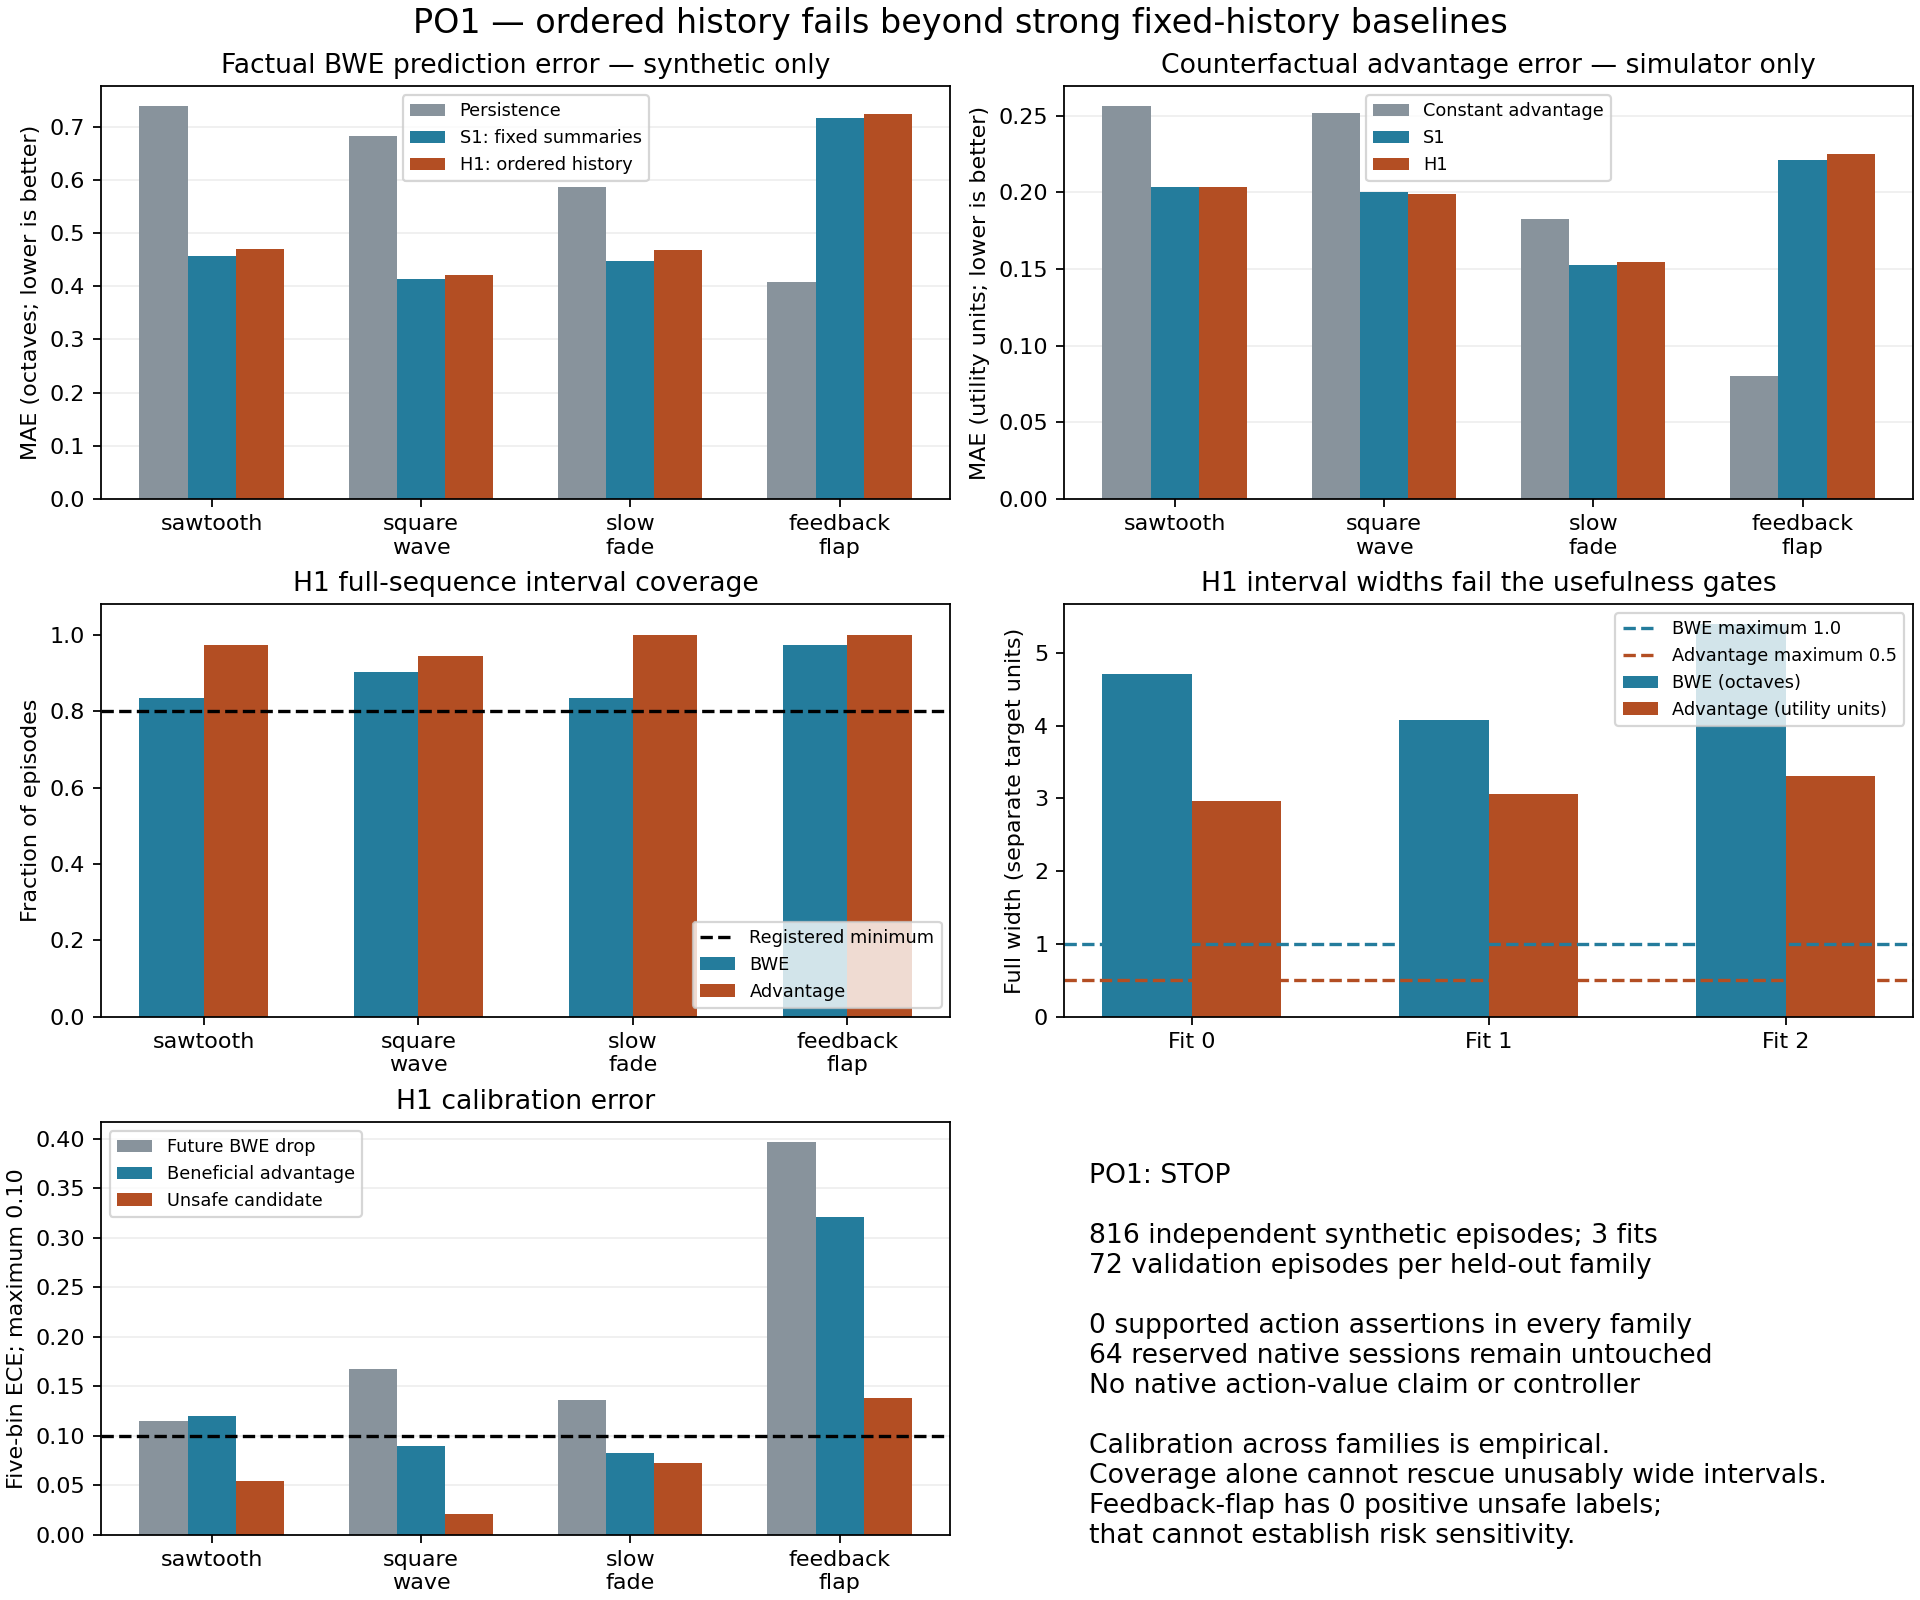
\includegraphics[width=\textwidth]{partial-observability-po1.png}
\caption{Frozen PO1 metrics from its committed report, with no new analysis.
Baseline comparisons, calibration error and interval widths must be read
alongside coverage. All families fail the preregistered conjunction. Families,
fits and decisions are not independent simulator implementations or native
replications.}
\label{fig:po1}
\end{figure}
\clearpage

\section{Scientific stopping decision}
\label{sec:decision}
% claim: stop
The active fine-grained learned native-control objective is closed under the
available fixture/data assumptions. No tested state passed its prospective
support contract; the mechanism route reached an observability boundary; the
new fixture was not admitted; PO1 did not supply robust predictive discrimination
or useful uncertainty. These failures cannot be repaired by pooling sources,
relaxing calipers, opening unused allocations, extending waits, increasing model
complexity or searching closed validation. The PO1 stop remains exact: no history
expansion, retraining with more complex sequence models, calibration/threshold
tuning, native factual panel, controller fit or safe-policy efficacy work from
that representation~\cite{rd1,po1}.

The untested causal role of transport timing and scientific value of an unbuilt
instrumented fixture remain unresolved. They limit the current conclusion;
they are not evidence that another experiment would succeed. RD1's conditional
discussion remains in its frozen decision document. This paper selects and
proposes no successor. The publication outcome is the bounded negative result.

\section{Limitations and nonclaims}
\label{sec:limits}
% claim: limitations
These are adaptive research questions with prospectively frozen individual
studies, not one preregistered omnibus experiment. Their sample counts cannot
be summed into a population confidence claim. Generated scenes, reused clips,
directions/windows, repeated landmarks and controlled inputs stay within their
source/campaign clusters. PSNR and 150 ms frame-readback delivery are local
proxies, not human QoE or live deployment safety. Technical qualification does
not establish an empty end-to-end path queue or complete estimator observability.

% claim: instrumentation_failures
Specific initial instrumentation failures remain failures: M6's 252 failed
development-clock cutoff bounds (not 252 native sessions); M7's four scheduler
originals, including 39/104 early service commands; M7R's four launcher attempts
and zero native sessions; M9's two excessive-gap originals among 64 validation
captures; M10's four cleanup overruns; and M11's two originals with SSRC0
configuration identity~\cite{m6,m7,m7r,m9,m10,m11}. Prospective repairs use fresh
captures without changing numerical gates. None is recast as a scientific null
or erased by a repair. IF1 was unattempted at build stage. P2 emitted no tags.
Neither circumstance supplies evidence for a zero mechanism effect.

% claim: nonclaims
We have not proved permanent history memory, universal nonsettling, causal
mediation by an internal queue, impossibility of instrumented Chromium, or a
general inability to identify randomized native policy effects. Synthetic
calibration failure is not native calibration failure; no PO1 native prediction
was measured. Conversely, a bounded positive simulator or local native estimate
does not establish broad native control value. The missing evidence is not
replaced with a stronger claim.

\section{Conclusion}
% claim: conclusion
Native early-service history has a qualified finite-horizon causal effect.
Local randomized action and policy contrasts can be measured, including a
harmful threshold policy. Yet the registered route to reproducible native
conditional value did not qualify. Current diagnostics leave internal timing
unobserved for causal online use; the instrumented build was never attempted;
the compact synthetic history screen failed robust action discrimination and
useful calibrated uncertainty under family shift. Together these results justify
stopping the current fine-grained learned-controller objective under the
available fixture and data assumptions. RD1 is the scientific stopping decision.
All frozen evidence and untouched allocations remain intact. No reserved panel
is opened, no successor is created and no model or controller is fitted or promoted.

\appendix
\section{Reproducibility and provenance}
% claim: provenance
RD1's machine-readable evidence ledger is
\path{data/research-decision-rd1/evidence-ledger.json}; its prior-file freeze is
\path{data/research-decision-rd1/prior-freeze-sha256.json}. RD1 sources, PDF and
audit are preserved in a private immutable archive whose receipt records fresh
object/member size and SHA-256 verification. This publication pass reads
committed summaries, not raw native captures. It does not register an experiment.

The paragraph-level source map is
\path{data/publication-readiness-rd1/claim-traceability.json}; verification is
recorded in \path{reports/publication-readiness-rd1-audit.json}. All 1,698 files
tracked at publication baseline \texttt{02c3693}, including RD1's decision,
source edition, reports, receipts and PDF, remain byte-identical. Publication
sources and PDF are in \path{paper/negative-result-publication/}. All project
reports cited here are pinned in the
\href{https://github.com/p-yan-6908/networkRLCD/tree/050e4f4be9b5135628cffb82e08821bbed143786}{public RD1 source tree at \texttt{050e4f4}}.
Private raw
access is restricted; committed reports and source locators support the numerical
claims without implying that raw native data or licensed media are public.

% Project reports below are pinned by the publication source map at 050e4f4.
\begin{thebibliography}{30}
\raggedright
\bibitem{rd1} networkRLCD. Research-decision synthesis RD1. Scientific stopping
decision, commit \texttt{050e4f4}.
\path{docs/RESEARCH_DECISION_RD1.md};
\path{data/research-decision-rd1/evidence-ledger.json}.
\bibitem{rfc8836} R. Jesup and Z. Sarker. Congestion Control Requirements for
Interactive Real-Time Media. RFC 8836, 2021. doi:10.17487/RFC8836.
\bibitem{ovadia} Y. Ovadia et al. Can You Trust Your Model's Uncertainty?
Evaluating Predictive Uncertainty Under Dataset Shift. NeurIPS, 2019.
\bibitem{scoring} T. Gneiting and A. E. Raftery. Strictly Proper Scoring Rules,
Prediction, and Estimation. JASA 102(477):359--378, 2007.
\bibitem{gcc} S. Holmer et al. A Google Congestion Control Algorithm for
Real-Time Communication. IETF draft-ietf-rmcat-gcc-02, 2016. Work in progress;
the simulator is not production libwebrtc.
\bibitem{earlier} networkRLCD. RLCD: Calibrated Reinforcement Learning for Safe
Real-Time Media Adaptation. Earlier frozen working manuscript at commit
\texttt{f109ab2}; \path{paper/main.tex}. Historical simulator results retain their
original scope; this negative-result edition supplies the current decision.
\bibitem{v9} networkRLCD. Native clock/action TURN/TCP V9 results. Frozen report.
\path{docs/NATIVE_CLOCK_ACTION_TURN_TCP_V9_RESULTS.md}.
\bibitem{v10} networkRLCD. Native clock/action TURN/TCP V10 results. Frozen report.
\path{docs/NATIVE_CLOCK_ACTION_TURN_TCP_V10_RESULTS.md}.
\bibitem{v11d} networkRLCD. Native clock/action V11D results. Frozen report.
\path{docs/NATIVE_CLOCK_ACTION_TURN_TCP_V11D_RESULTS.md}.
\bibitem{v12} networkRLCD. V12 execution: support qualification failed. Frozen report.
\path{docs/NATIVE_SUPPORT_VALIDATION_V12_RESULTS.md}.
\bibitem{v13} networkRLCD. V13 execution: support failed; action study closed.
\path{docs/NATIVE_CONTINUOUS_VALIDATION_V13_RESULTS.md}.
\bibitem{m5} networkRLCD. M5: qualified instrumentation makes the prefix-history
effect estimable. \path{docs/NATIVE_PREFIX_MEMORY_M5_RESULTS.md}.
\bibitem{m6r} networkRLCD. M6R: history-state common support did not qualify.
\path{docs/NATIVE_HISTORY_STATE_M6R_RESULTS.md}.
\bibitem{m6} networkRLCD. M6: pre-selection temporal-mapping guard failure.
\path{docs/NATIVE_HISTORY_STATE_M6_CLOSURE.md}.
\bibitem{m7} networkRLCD. M7: instrumentation-limited feasibility failure.
\path{docs/NATIVE_STATE_CONDITIONING_M7_RESULTS.md}.
\bibitem{m7r} networkRLCD. M7R: launcher failure before native instrumentation.
\path{docs/NATIVE_STATE_CONDITIONING_M7R_RESULTS.md}.
\bibitem{m7ra} networkRLCD. M7RA: qualified instrumentation, failed prospective
state creation. \path{docs/NATIVE_STATE_CONDITIONING_M7RA_RESULTS.md}.
\bibitem{m8} networkRLCD. M8: native BWE response to controlled service.
\path{docs/NATIVE_BWE_TRANSIENTS_M8_RESULTS.md}.
\bibitem{m9r} networkRLCD. M9R: prospective phase-aware state and longer-horizon
stability; interpretation and registered residual audit.
\path{docs/NATIVE_PHASE_STATE_M9R_RESULTS.md};
\path{docs/NATIVE_PHASE_STATE_M9R_INTERPRETATION.md}.
\bibitem{m9} networkRLCD. M9: instrumentation-limited phase-state validation.
\path{docs/NATIVE_PHASE_STATE_M9_RESULTS.md}.
\bibitem{m10r} networkRLCD. M10R: fresh causal mechanism observability assay;
qualified observability, mechanism discrimination not established.
\path{docs/NATIVE_MECHANISM_OBSERVABILITY_M10R_RESULTS.md};
\path{docs/NATIVE_MECHANISM_OBSERVABILITY_M10R_INTERPRETATION.md}.
\bibitem{m10} networkRLCD. M10: cleanup instrumentation-limited stop.
\path{docs/NATIVE_MECHANISM_OBSERVABILITY_M10_RESULTS.md}.
\bibitem{m11r} networkRLCD. M11R: transport-control timing did not qualify for
causal use. \path{docs/NATIVE_TRANSPORT_TIMING_M11R_RESULTS.md}.
\bibitem{m11} networkRLCD. M11: sender-identity instrumentation limitation.
\path{docs/NATIVE_TRANSPORT_TIMING_M11_RESULTS.md}.
\bibitem{if1} networkRLCD. IF1: registered instrumented-fixture plan; build
admission failed. \path{docs/NATIVE_INSTRUMENTED_FIXTURE_IF1_RESULT.md}.
\bibitem{po1} networkRLCD. PO1: bounded observable-history information screen;
result: stop the bounded history-information route. Registration \texttt{d43d407},
result \texttt{f109ab2}.
\path{docs/PARTIAL_OBSERVABILITY_PO1_PLAN.md};
\path{docs/PARTIAL_OBSERVABILITY_PO1_RESULTS.md}.
\end{thebibliography}

\end{document}
